
\de{ĐỀ THI GIỮA HỌC KỲ I NĂM HỌC 2022-2023}{THPT Nguyễn Thái Bình}


\Opensolutionfile{ans}[ans/ans]

\Opensolutionfile{ans}[ans/ans-NTB-TP.HCM-2022]
	\begin{ex}%[Đề GHK2, THPT Nguyễn Thái Bình-TPHCM-BC Tuan]%[0T2Y1-1]
	Bất phương trình nào sau đây là bất phương trình bậc nhất hai ẩn?
	\choice
	{\True $-3x+2y-5 \ge 0$}
	{$3x^2-2y+1>0$}
	{$(x-y)(2x+5y)<0$}
	{$3x^2-2y+5 \ge 0$}
	\loigiai{
		Ta có $-3x+2y-5 \ge 0$ là bất phương trình bậc nhất theo $2$ ẩn $x$ và $y$.
	}
\end{ex}

\begin{ex}%[Đề GHK2, THPT Nguyễn Thái Bình-TPHCM-BC Tuan]%[0T4Y1-1]
	Nếu $\alpha$ là góc tù thì khẳng định nào \textbf{sai}?
	\choice
	{$\tan\alpha<0$}
	{$\cot\alpha<0$}
	{$\cos\alpha<0$}
	{\True $\sin\alpha<0$}
	\loigiai{
		Với mọi góc $\alpha$ thoả mãn $0^{\circ} \le \alpha \le 180^{\circ}$ ta có $\sin\alpha \ge 0$ nên \lq\lq $\sin\alpha<0$ khi $\alpha$ tù\rq\rq\ là sai.
	}
\end{ex}

\begin{ex}%[Đề GHK2, THPT Nguyễn Thái Bình-TPHCM-BC Tuan]%[0T1Y1-2]
	Trong các phát biểu sau, phát biểu nào là mệnh đề đúng?
	\choice
	{Hình chữ nhật có hai đường chéo vuông góc}
	{\True $5$ là số hữu tỉ}
	{$\pi$ là số tự nhiên}
	{Tam giác có một góc bằng $60^{\circ}$ là tam giác đều}
	\loigiai{
		Ta có \lq\lq $5$ là số hữu tỉ\rq\rq\ là mệnh đề đúng.
	}
\end{ex}

\begin{ex}%[Đề GHK2, THPT Nguyễn Thái Bình-TPHCM-BC Tuan]%[0T1B3-1]
	Cho $M=\big\{0;1;2;3\big\}$, $N=\big\{0;3;4;5;6\big\}$. Khẳng định nào sau đây đúng?
	\choice
	{$M \cap N=\big\{4;5;6\big\}$}
	{$M \cap N=\big\{0;1;2;3;4;5;6\big\}$}
	{\True $M \cap N=\big\{0;3\big\}$}
	{$M \cap N=\big\{1;2\big\}$}
	\loigiai{
		Ta có $\big\{0;1;2;3\big\} \cap \big\{0;3;4;5;6\big\}=\big\{0;3\big\}$.
	}
\end{ex}

\begin{ex}%[Đề GHK2, THPT Nguyễn Thái Bình-TPHCM-BC Tuan]%[0T3B1-1]
	Cho hàm số $f(x)=\heva{&2x^2-3x+1 &&\text{khi } x \leq 2\\&-3x+4&&\text{khi } x>2}$. Giá trị $f(2)$ bằng
	\choice
	{$-2$}
	{$0$}
	{$1$}
	{\True $3$}
	\loigiai{
		Với $x=2$ ta dùng công thức $f(x)=2x^2-3x+1$ do đó $f(2)=2\cdot 2^2-3\cdot 2+1=3$.}
\end{ex}

\begin{ex}%[Đề GHK2, THPT Nguyễn Thái Bình-TPHCM-BC Tuan]%[0T3Y1-1]
	\immini{
		Nhiệt độ vào lúc $13$ giờ là
		\choice
		{\True $31^{\circ}\mathrm{C}$}
		{$27^{\circ}\mathrm{C}$}
		{$29^{\circ}\mathrm{C}$}
		{$28^{\circ}\mathrm{C}$}}
	{\vspace{-0.5cm}
		\begin{tikzpicture}[scale=0.97,line cap=round]
			\begin{scope}[scale=0.678,shift={(-8.82,-1.91)}]
				\draw[gray,line width=2.5pt] (-1.9,-1.7) rectangle (8.55,5.5);
				\draw[fill=cyan!30] (-1.9,-1.7) rectangle (8.55,5.5);
				\node at (3.3,4.74){\fontsize{8.5}{0}\selectfont\textbf{Dự báo nhiệt độ ngày 01/5/2021}};
				\node at (3.3,4.18){\scriptsize\textbf{tại Thành phố Hồ Chí Minh}};
				\node at (-1.45,1.8)[rotate=90]{\fontsize{8.}{0}\selectfont\textbf{Nhiệt độ} ($^{\circ}$C)};
				\foreach \y in {0,1,2,...,5}{
					\pgfmathsetmacro{\s}{int(\y*2+24)};
					\node at (-0.8,\y*0.738){\footnotesize$\s$};}
				\fill[white] (0,0) rectangle (8,3.69);
				\draw[xstep=8,ystep=3.69/5,gray!50] (0,0) grid (8,3.69);
				\draw[thick] (0,0) rectangle (8,3.69);
				\foreach \x\y\t in {0.5/1.476/A,1.5/1.107/B,2.5/1.476/C,3.5/2.952/D,4.5/2.583/E,5.5/1.845/F,6.5/1.476/G,7.5/1.107/H}
				\coordinate (\t) at (\x,\y);
				\draw[line width=1.5pt] (A)--(B)--(C)--(D)--(E)--(F)--(G)--(H);
				\foreach \t/\s in {A/28,B/27,C/28,D/32,E/31,F/29,G/28,H/27}
				\draw[fill=black] (\t)circle(1.2mm) +(90:12pt)node{\footnotesize $\s$};
				\foreach \x in {1,2,3,...,8}{
					\draw[thick,red] (0,-0.17)|-(\x-0.5,0)--(\x-0.5,-0.17);
					\pgfmathsetmacro{\s}{int(\x*3-2)};
					\node at (\x-0.5,-0.7){\footnotesize$\s$};}
				\node at (4,-1.3){\scriptsize\textbf{Giờ}};
			\end{scope}
	\end{tikzpicture}}
	\loigiai{
		Theo biểu đồ nhiệt độ vào lúc $13$ giờ là $31^{\circ}\mathrm{C}$.
	}
\end{ex}

\begin{ex}%[Đề GHK2, THPT Nguyễn Thái Bình-TPHCM-BC Tuan]%[0T3B2-1]
	Bảng biến thiên của hàm số $y=-2x^2+4x+1$ là bảng nào sau đây?
	\def\dotEX{}
	\choice
	{
\begin{tikzpicture}
			\tkzTabInit[nocadre=true,lgt=1.2,espcl=2.5,deltacl=0.6]
			{$x$/0.6,$y$/2}
			{$-\infty$,$1$,$+\infty$}
			\tkzTabVar{+/$+\infty$,-/$3$,+/$+\infty$}
		\end{tikzpicture}
	}
	{\True 
\begin{tikzpicture}
			\tkzTabInit[nocadre=true,lgt=1.2,espcl=2.5,deltacl=0.6]
			{$x$/0.6,$y$/2}
			{$-\infty$,$1$,$+\infty$}
			\tkzTabVar{-/$-\infty$,+/$3$,-/$-\infty$}
	\end{tikzpicture}}
	{
\begin{tikzpicture}
			\tkzTabInit[nocadre=true,lgt=1.2,espcl=2.5,deltacl=0.6]
			{$x$/0.6,$y$/2}
			{$-\infty$,$2$,$+\infty$}
			\tkzTabVar{-/$-\infty$,+/$1$,-/$-\infty$}
	\end{tikzpicture}}
	{
\begin{tikzpicture}
			\tkzTabInit[nocadre=true,lgt=1.2,espcl=2.5,deltacl=0.6]
			{$x$/0.6,$y$/2}
			{$-\infty$,$2$,$+\infty$}
			\tkzTabVar{+/$+\infty$,-/$1$,+/$+\infty$}
	\end{tikzpicture}}
	\loigiai{
		Parabol $y=-2x^2+4x+1$ có toạ độ đỉnh $I(1;3)$ và có $a=-2<0$ nên hướng bề lõm quay xuống dưới.
	}
\end{ex}

\begin{ex}%[Đề GHK2, THPT Nguyễn Thái Bình-TPHCM-BC Tuan]%[0T4Y2-1]
	Cho tam giác $ABC$ với $BC=a$, $AC=b$, $AB=c$. Công thức nào sau đây đúng?
	\choice
	{$b^2=a^2+c^2-2ac\cos A$}
	{$b^2=a^2+c^2-2ac\cos C$}
	{\True $b^2=a^2+c^2-2ac\cos B$}
	{$b^2=a^2+c^2+2ac\cos B$}
	\loigiai{
		Theo định lý cô-sin ta có $b^2=a^2+c^2-2ac\cos B$.
	}
\end{ex}

\begin{ex}%[Đề GHK2, THPT Nguyễn Thái Bình-TPHCM-BC Tuan]%[0T1B2-1]
	Viết tập hợp $X=\big\{0;1;2;3;4\big\}$ dưới dạng chỉ ra tính chất đặc trung cho các phần tử.
	\choice
	{$X=\big\{x \in \mathbb{Z}\mid x \leq 4\big\}$}
	{$X=\big\{x \in \mathbb{N}^* \mid x \leq 4\big\}$}
	{$X=\big\{x \in \mathbb{Q}\mid x \leq 4\big\}$}
	{\True $X=\big\{x \in \mathbb{N}\mid x \leq 4\big\}$}
	\loigiai{
		Ta có $0;1;2;3;4$ là các số tự nhiên không vượt quá $4$ nên $X=\big\{x \in \mathbb{N}\mid x \leq 4\big\}$.
	}
\end{ex}

\begin{ex}%[Đề GHK2, THPT Nguyễn Thái Bình-TPHCM]%[0T4Y2-1]
	Cho tam giác $ABC$ có bán kính đường tròn ngoại tiếp tam giác là $R$ và $BC=a$. Mệnh đề nào dưới đây đúng?
	\choice
	{$\dfrac{a}{\sin A}=3R$}
	{\True $\dfrac{a}{\sin A}=2R$}
	{$\dfrac{a}{\sin A}=R$}
	{$\dfrac{a}{\sin A}=4R$}
	\loigiai{
		Theo định lý sin ta có $\dfrac{a}{\sin A}=2R$.
	}
\end{ex}

	%%CÂU 11
	\begin{ex}%[Đề GHK2, THPT Nguyễn Thái Bình-TPHCM-Vu Ngoc Hao]%[0T1Y2-1]
		Cho tập hợp $M=\big\{x \in \mathbb{N} \mid x < 4\big\}$. Tìm mệnh đề đúng.
		\choice
		{$M=\big\{0;1;2;3;4\big\}$}
		{\True $M=\big\{0;1;2;3\big\}$}
		{$M=\big\{4\big\}$}
		{$M=\big\{1;2;3\big\}$}
		\loigiai{
			Các số tự nhiên $x<4$ bao gồm $0;1;2;3$ do đó $M=\big\{0;1;2;3\big\}$.
		}
	\end{ex}
	%%CÂU 12
	\begin{ex}%[Đề GHK2, THPT Nguyễn Thái Bình-TPHCM-Vu Ngoc Hao]%[0T4Y1-2]
		Với mỗi góc $\alpha$ $\left(0^{\circ} \leq \alpha \leq 
		180^{\circ}\right)$, ta xác định được một điểm $M$ duy nhất trên nửa 
		đường tròn đơn vị sao cho $\widehat{xOM}=\alpha$. Gọi $(x_0;y_0)$ là 
		toạ độ điểm $M$, ta có
		\choice
		{$\tan\alpha=\dfrac{x_0}{y_0}$ $\left(y_0 \neq 0\right)$}
		{$\cot\alpha=\dfrac{y_0}{x_0}$ $\left(x_0 \neq 0\right)$}
		{$\sin\alpha=x_0$}
		{\True $\cos\alpha=x_0$}
		\loigiai{
			Theo định nghĩa các giá trị lượng giác của góc $\alpha$ ta có $\cos\alpha=x_0$.
		}
	\end{ex}
		%%CÂU 13
	\begin{ex}%[Đề GHK2, THPT Nguyễn Thái Bình-TPHCM-Vu Ngoc Hao]%[0T3Y2-2]
		Hàm số nào trong các hàm số sau đây là hàm số bậc hai?
		\choice
		{$y=-4x^3+3x^2-1$}
		{\True $y=-5x^2+3x-8$}
		{$y=\sqrt{2x^2+x-1}$}
		{$y=\dfrac{-x^2+3x-1}{x^2+x+1}$}
		\loigiai{
			Hàm số $y=-5x^2+3x-8$ là hàm số bậc hai với các hệ số $a=-5$, $b=3$, $c=-8$.
		}
	\end{ex}
		%%CÂU 14
	\begin{ex}%[Đề GHK2, THPT Nguyễn Thái Bình-TPHCM-Vu Ngoc Hao]%[0T1B1-4]
		Cho định lí dạng $P \Rightarrow Q$. Phát biểu nào sau đây đúng?
		\choice
		{$P$ là kết luận của định lí}
		{$Q$ là giả thiết của định lí}
		{\True $Q$ là điều kiện cần để có $P$}
		{$Q$ là điều kiện đủ để có $P$}
		\loigiai{
			Trong mệnh đề $P \Rightarrow Q$ ta phát biểu \lq\lq$Q$ là điều kiện 
			cần để có $P$\rq\rq.
		}
	\end{ex}
	%%CÂU 15
	\begin{ex}%[Đề GHK2, THPT Nguyễn Thái Bình-TPHCM-Vu Ngoc Hao]%[0T2Y1-2]
		Cặp số nào sau đây là nghiệm của bất phương trình $-3x+5y \leq 6$?
		\choice
		{$(2;8)$}
		{\True $(3;3)$}
		{$(-10;-3)$}
		{$(0;2)$}
		\loigiai{
			Lần lượt thay các cặp số vào bất phương trình ta chỉ được mệnh đề 
			đúng là \lq\lq$-3\cdot 3+5\cdot 3 \leq 6$\rq\rq.
		}
	\end{ex}
		%%CÂU 16
	\begin{ex}%[Đề GHK2, THPT Nguyễn Thái Bình-TPHCM-Vu Ngoc Hao]%[0T4B2-1]
		Tam giác $ABC$ có $AB=8$, $BC=15$, $CA=13$. Số đo góc $\widehat{B}$ bằng
		\choice
		{$90^{\circ}$}
		{\True $60^{\circ}$}
		{$45^{\circ}$}
		{$30^{\circ}$}
		\loigiai{
			Với $AB=c=8$, $BC=a=15$, $CA=b=13$ ta có 
			$$\cos B=\dfrac{a^2+c^2-b^2}{2ac}=\dfrac{15^2+8^2-13^2}{2\cdot 15 \cdot 8}=\dfrac{1}{2} 
			\Rightarrow \widehat{B}=60^{\circ}.$$
		}
	\end{ex}
		%%CÂU 17
	\begin{ex}%[Đề GHK2, THPT Nguyễn Thái Bình-TPHCM-Vu Ngoc Hao]%[0T1B1-4]
		Sử dụng thuật ngữ \lq\lq\textit{điều kiện cần}\rq\rq \; để phát biểu 
		lại 
		định lí: \lq\lq Nếu tứ giác $ABCD$ là hình thoi thì hai đường chéo 
		vuông góc\rq\rq.
		\choice
		{Tứ giác $ABCD$ là hình thoi là điều kiện cần để tứ giác này có hai đường chéo vuông góc}
		{\True Tứ giác $ABCD$ có hai đường chéo vuông góc là điều kiện cần để tứ giác này là hình thoi}
		{Tứ giác $ABCD$ có hai đường chéo vuông góc là điều kiện đủ để tứ giác này là hình thoi}
		{Tứ giác $ABCD$ là hình thoi là điều kiện cần và đủ để hai đường chéo của tứ giác này vuông góc}
		\loigiai{
			Định lí: \lq\lq Nếu tứ giác $ABCD$ là hình thoi thì hai đường chéo 
			vuông góc\rq\rq \; là một mệnh đề kéo theo.\\
			Và cách phát biểu khác của nó là: \lq\lq Tứ giác $ABCD$ có hai 
			đường chéo vuông góc là điều kiện cần để tứ giác này là hình 
			thoi\rq\rq.
		}
	\end{ex}
		%%CÂU 18
	\begin{ex}%[Đề GHK2, THPT Nguyễn Thái Bình-TPHCM-Vu Ngoc Hao]%[0T1Y3-1]
		Cho hai tập hợp $E$ và $F$ có biểu đồ Ven như hình vẽ. 
		\immini{
			Hãy xác định tập hợp $E \cap F$.
			\choice
			{$E \cap F=\big\{3;4;5\big\}$}
			{\True $E \cap F=\big\{1;2\big\}$}
			{$E \cap F=\big\{1;2;3;4;5;7;9;11\big\}$}
			{$E \cap F=\big\{7;9;11\big\}$}}
		{\vspace{-0.5cm}
			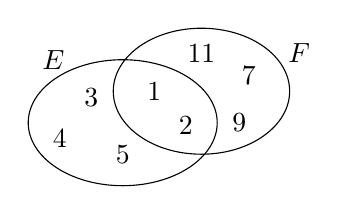
\begin{tikzpicture}[scale=0.4]
			\def\firstven{(0,0) ellipse (3cm and 2cm)}
			\def\secondven{(2.5,1) ellipse (2.8cm and 2cm)}
			\draw \firstven \secondven;
			\node at (-2.2,2) {$E$};
			\node at (5.6,2.2){$F$};
			\node at (1,1){$1$};
			\node at (2,-0.1){$2$};
			\node at (-1,0.8){$3$};
			\node at (-2,-0.5){$4$};
			\node at (0,-1){$5$};
			\node at (2.5,2.2){$11$};
			\node at (4,1.5){$7$};
			\node at (3.7,0){$9$};
			\end{tikzpicture}}
		\loigiai{
			Theo biểu đồ Ven ta có $E \cap F=\big\{1;2\big\}$.
		}
	\end{ex}
		%%CÂU 19
	\begin{ex}%[Đề GHK2, THPT Nguyễn Thái Bình-TPHCM-Vu Ngoc Hao]%[0T3B2-1]
		Tung độ đỉnh $I$ của parabol $(P)\colon y=2x^2+8x-7$ là
		\choice
		{\True $-15$}
		{$15$}
		{$-5$}
		{$5$}
		\loigiai{
			Parabol $(P)\colon y=2x^2+8x-7$ có hoành độ đỉnh là 
			$x_I=-\dfrac{8}{2\cdot 2}=-2$ nên có tung độ đỉnh là 
			$y_I=2(-2)^2+8(-2)-7=-15$.
		}
	\end{ex}
	%%CÂU 20
	\begin{ex}%[Đề GHK2, THPT Nguyễn Thái Bình-TPHCM-Vu Ngoc Hao]%[0T1B3-5]
		Cho hai tập hợp $X=(-\infty;1)$, $Y=[0;5)$. Chọn khẳng định đúng trong các khẳng định sau đây.
		\choice
		{$X \cup Y=(1;5]$}
		{\True $X \cup Y=(-\infty;5)$}
		{$X \cup Y=\mathbb{R}$}
		{$X \cup Y=(1;5)$}
		\loigiai{
			Ta có $X \cup Y=(-\infty;1) \cup [0;5)=(-\infty;5)$.
		}
	\end{ex}
	
\begin{ex}%[0D1Y2-3]%[Dự án đề kiểm tra HKII NH22-23- Nguyễn Ngọc Dũng]%[THPT Nguyễn Thái Bình]
Hình vẽ dưới đây (phần không bi gạch chéo) biểu diễn cho tập hợp nào?
\begin{center}
\begin{tikzpicture}[>=stealth]
\draw[->](-4,0)->(3,0);
\def\skipInterval{0.4cm}
\def\colorInterval{blue}
\IntervalLR{-4}{-2}\IntervalGRF{}{}{[}{-2}
\IntervalLR{1}{3}\IntervalGRF{)}{1}{}{}
\end{tikzpicture}
\end{center}
\choice
{$(-\infty;-2] \cup [1;+\infty)$}
{$[-2;1]$}
{$(-\infty;-2] \cup (1;+\infty)$}
{\True $[-2;1)$}
\loigiai{
Hình vẽ trên trục số biểu diễn cho nửa khoảng $[-2;1)$.
}
\end{ex}

\begin{ex}%[0D1Y1-3]%[Dự án đề kiểm tra HKII NH22-23- Nguyễn Ngọc Dũng]%[THPT Nguyễn Thái Bình]
Cho mệnh đề $P\colon {\lq\lq}\pi \text{ là một số vô tỉ\rq\rq}$. Mệnh đề nào sau đây là mệnh đề phủ định của $P$?
\choice
{\True {\lq\lq}$\pi$ không là một số vô tỉ{\rq\rq}}
{{\lq\lq}$\pi$ không là một số thực{\rq\rq}}
{{\lq\lq}$\pi$ không là một số hữu tỉ{\rq\rq}}
{{\lq\lq}$\pi$ là một số vô tỉ{\rq\rq}}
\loigiai{
Với $P\colon {\lq\lq}\pi\text{ là một số vô tỉ{\rq\rq}}$ thì phủ định của $P$ là $\overline{P}\colon {\lq\lq}\pi\text{ không là một số vô tỉ{\rq\rq}}$.
}
\end{ex}

\begin{ex}%[0H4Y2-1]%[Dự án đề kiểm tra HKII NH22-23- Nguyễn Ngọc Dũng]%[THPT Nguyễn Thái Bình]
Cho tam giác $ABC$ có $AB=6$, $AC=4$, $\widehat{A}=120^{\circ}$. Độ dài cạnh $BC$ bằng
\choice
{$2\sqrt{7}$}
{$\sqrt{19}$}
{\True $2\sqrt{19}$}
{$3\sqrt{19}$}
\loigiai{
Ta có $AB=c=6$, $AC=b=4$, $\widehat{A}=120^{\circ}$ nên
$$a^2=b^2+c^2-2bc\cos A=4^2+6^2-2\cdot 4\cdot 6\cdot\cos 120^{\circ}=76 
\Rightarrow BC=a=\sqrt{76}=2\sqrt{19}.$$
}
\end{ex}

\begin{ex}%[0H4B1-2]%[Dự án đề kiểm tra HKII NH22-23- Nguyễn Ngọc Dũng]%[THPT Nguyễn Thái Bình]
Biết $\cos\alpha=-\dfrac{2}{3}$ với $90^{\circ}<\alpha<180^{\circ}$. Khẳng định nào \textbf{sai}?
\choice
{$\sin^2\alpha+\cos^2\alpha=1$}
{$\cos\left(180^{\circ}-\alpha\right)=\dfrac{2}{3}$}
{$\sin\left(90^{\circ}-\alpha\right)=-\dfrac{2}{3}$}
{\True $\sin\left(90^{\circ}-\alpha\right)=\dfrac{2}{3}$}
\loigiai{
Ta có $\sin\left(90^{\circ}-\alpha\right)=\cos\alpha=-\dfrac{2}{3}$ do đó $\sin\left(90^{\circ}-\alpha\right)=\dfrac{2}{3}$ là khẳng định sai.\\
Các khẳng định còn lại đều đúng.
}
\end{ex}

\begin{ex}%[0D3Y1-2]%[Dự án đề kiểm tra HKII NH22-23- Nguyễn Ngọc Dũng]%[THPT Nguyễn Thái Bình]
Tập xác định $\mathscr{D}$ của hàm số $f(x)=\sqrt{2x+4}$ là
\choice
{\True $\mathscr{D}=[-2;+\infty)$}
{$\mathscr{D}=(-2;+\infty)$}
{$\mathscr{D}=(-\infty;-2]$}
{$\mathscr{D}=\mathbb{R}$}
\loigiai{
Hàm số $f(x)=\sqrt{2x+4}$ có nghĩa khi và chỉ khi $2x+4 \geq 0 \Leftrightarrow x \geq -2$.\\
Suy ra tập xác định $\mathscr{D}$ của hàm số $f(x)=\sqrt{2x+4}$ là $\mathscr{D}=[-2;+\infty)$
}
\end{ex}

\begin{ex}%[0D2B1-3]%[Dự án đề kiểm tra HKII NH22-23- Nguyễn Ngọc Dũng]%[THPT Nguyễn Thái Bình]
Miền nghiệm của bất phương trình $x-2y<4$ được xác định bởi miền nào (nửa mặt phẳng không bị gạch và không kẻ bờ $d$) sau đây?
\choice
{\begin{tikzpicture}[line join=round, line cap=round,>=stealth,thick]
\tikzset{every node/.style={scale=0.9}}
\begin{scope}
\clip (-3,-1) rectangle (2,5);
\fill[pattern=north east lines] (-5,-6)--(-5,10)--(3,10)--cycle;
\draw (0.5,5)--(-2.5,-1);
\draw[->] (-4,0)--(2,0) node[below]{$x$};
\draw[->] (0,-1)--(0,5) node[left]{$y$};
\draw (0,0) node[below left]{$O$};
\path 
(-2,0)node[below right]{$-2$}
(0,4)node[right]{$4$}
;
\end{scope}
\end{tikzpicture}}
{\begin{tikzpicture}[line join=round, line cap=round,>=stealth,thick]
\tikzset{every node/.style={scale=0.9}}
\begin{scope}
\clip (-2.3,-1) rectangle (2,5);
\fill[pattern=north east lines] (-5,-6)--(3,-6)--(3,10)--cycle;
\draw (0.5,5)--(-2.5,-1);
\draw[->] (-4,0)--(2,0) node[below]{$x$};
\draw[->] (0,-1)--(0,5) node[left]{$y$};
\draw (0,0) node[below left]{$O$};
\path 
(-2,0)node[above]{$-2$}
(0,4)node[left]{$4$}
;
\end{scope}	
\end{tikzpicture}}
{\begin{tikzpicture}[line join=round, line cap=round,>=stealth,thick]
\tikzset{every node/.style={scale=0.9}}
\begin{scope}
\clip (-1,-3) rectangle (5,2);
\fill[pattern=north east lines] (-3,-3.5)--(-3,2.5)--(9,2.5)--cycle;
\draw (8,2)--(-2,-3);
\draw[->] (-2,0)--(5,0) node[below]{$x$};
\draw[->] (0,-3)--(0,2) node[left]{$y$};
\draw (0,0) node[below left]{$O$};
\path 
(0,-2)node[right]{$-2$}
(4,0)node[below]{$4$}
;
\end{scope}
\end{tikzpicture}}
{\True \begin{tikzpicture}[line join=round, line cap=round,>=stealth,thick]
\tikzset{every node/.style={scale=0.9}}
\begin{scope}
\clip (-2,-3) rectangle (5,2);
\fill[pattern=north east lines] (-3,-3.5)--(9,-3.5)--(9,2.5)--cycle;
\draw (8,2)--(-2,-3);
\path 
(0,-2)node[right]{$-2$}
(4,0)node[below]{$4$}
;
\draw[->] (-2,0)--(5,0) node[below]{$x$};
\draw[->] (0,-3)--(0,2) node[left]{$y$};
\draw (0,0) node[below left]{$O$};
\end{scope}	
\end{tikzpicture}}
\loigiai{
Đường thẳng $d\colon x-2y=4$ đi qua hai điểm $(0;-2)$ và $(4;0)$.\\
Xét $O(0;0)\notin d$:\\ 
Thay $x=0$; $y=0$ vào bất phương trình $x-2y<4$ ta thấy đúng, suy ra miền nghiệm chứa $O(0;0)$.
}
\end{ex}

\begin{ex}%[0H4Y1-2]%[Dự án đề kiểm tra HKII NH22-23- Nguyễn Ngọc Dũng]%[THPT Nguyễn Thái Bình]
Hai góc $\alpha$ và $\beta$ phụ nhau, hệ thức nào sau đây là đúng?
\choice
{$\cos(\alpha+\beta)=1$}
{$\sin\beta=-\cos\alpha$}
{$\cot\alpha=-\tan\beta$}
{\True $\cos\alpha=\sin\beta$}
\loigiai{
Do $\alpha$ và $\beta$ phụ nhau nên $\cos\alpha=\sin\beta$.
}
\end{ex}

\begin{ex}%[0D3B1-4]%[Dự án đề kiểm tra HKII NH22-23- Nguyễn Ngọc Dũng]%[THPT Nguyễn Thái Bình]
Khoảng nghịch biến của hàm số có đồ thị sau là
\begin{center}
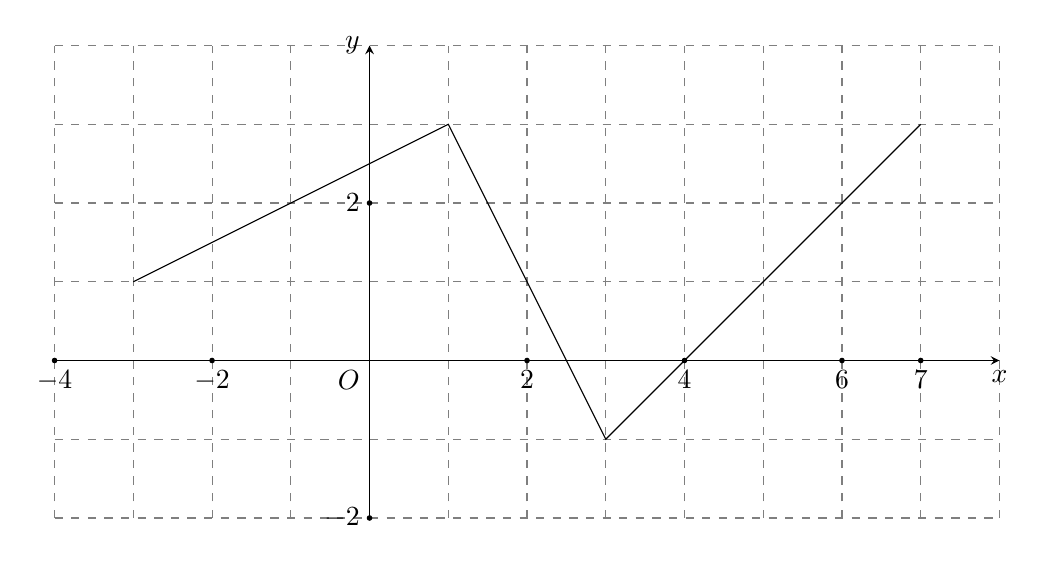
\begin{tikzpicture}
\draw[dashed,opacity=0.5] (-4,4)grid(8,-2);
\draw[-stealth] (-4,0)--(8,0)node[below]{$x$};
\draw[-stealth] (0,-2)--(0,4)node[left]{$y$};
\draw (-3,1)--(1,3)--(3,-1)--(7,3)
(0,0)node[below left]{$O$}
;
\foreach \i in{-4,-2,2,4,6,7}{\draw[fill=black] (\i,0)circle(0.8pt)node[below]{$\i$}; }
\foreach \i in{-2,2}{\draw[fill=black] (0,\i)circle(0.8pt)node[left]{$\i$}; }
\end{tikzpicture}
\end{center}
\choice
{$(-2;1)$}
{$(3;6)$}
{\True $(1;2)$}
{$(2;6)$}
\loigiai{Dựa vào đồ thị ta thấy khoảng nghịch biến của hàm số là $(1;2)$.}
\end{ex}

\begin{ex}%[0D3B2-1]%[Dự án đề kiểm tra HKII NH22-23- Nguyễn Ngọc Dũng]%[THPT Nguyễn Thái Bình]
Tìm điều kiện của $m$ để hàm số $y=2x^2-4x-m^2+4$ đạt giá trị nhỏ nhất bằng $3$.
\choice
{\True $m\in\varnothing$}
{$m\in\mathbb{R}$}
{$m\in\left\{-1;1\right\}$}
{$m=3$}
\loigiai{Đỉnh $I(2;4-m^2)$.\\
Bảng biến thiên
\begin{center}

\begin{tikzpicture}
\tkzTabInit[nocadre,lgt=1,espcl=3]{$x$/0.7,$y$/2.5}{$-\infty$,$2$,$+\infty$}
\tkzTabVar{+/$+\infty$,-/$4-m^2$,+/$+\infty$}
\end{tikzpicture}
\end{center}
Dựa vào bảng biến thiên suy ra hàm số đạt giá trị nhỏ nhất bằng $4-m^2$.\\
Suy ra $4-m^2=3\Leftrightarrow \hoac{&m=1\\&m=-1.}$
}
\end{ex}

\begin{ex}%[0D1K3-3]%[Dự án đề kiểm tra HKII NH22-23- Nguyễn Ngọc Dũng]%[THPT Nguyễn Thái Bình]
Một lớp học có $30$ học sinh giỏi môn Lý, $20$ học sinh giỏi môn Hóa, $10$ học sinh giỏi cả môn Hóa và Lý và có $4$ học sinh không giỏi môn nào cả. Hỏi lớp đó có bao nhiêu học sinh?
\choice
{\True $44$}
{$64$}
{$34$}
{$54$}
\loigiai{
Số học sinh chỉ giỏi Lý là $30-10=20$ học sinh.\\
Số học sinh chỉ giỏi Hóa là $20-10=10$ học sinh.\\
Vậy lớp đó có $20+10+4+10=44$ học sinh.
}
\end{ex}


\begin{ex}%[0T4B3-1]%[Dự án đề kiểm tra HKI NH22-23- Hieu Phan]%[THPT Nguyễn Thái Bình]
	Tam giác $ABC$ có $AB=13$, $AC=14$, $BC=15$. Tính diện tích tam giác $ABC$.
	\choice
	{$3\sqrt{3}$}
	{$42$}
	{$6\sqrt{3}$}
	{\True $84$}
	\loigiai{Ta có $p=\dfrac{AB+AC+BC}{2}=\dfrac{13+14+15}{2}=21$.\\
	Áp dụng công thức Hê-rông ta có\\
	\centerline{$S=\sqrt{p(p-AB)(p-AC)(p-BC)}=\sqrt{21(21-13)(21-14)(21-15)}=84$.}}
\end{ex}
\begin{ex}%[0T3B1-1]%[Dự án đề kiểm tra HKI NH22-23- Hieu Phan]%[THPT Nguyễn Thái Bình]
	\immini[thm]
	{Điểm nào thuộc đồ thị $(P)$ của hàm số bậc $2$ đã cho
		\choice
		{$(0;2)$}
		{$(1;1)$}
		{$(4;1)$}
		{\True $(2;-1)$}}
	{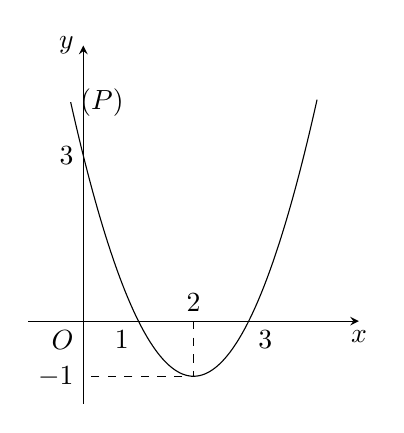
\begin{tikzpicture}[>=stealth,scale=0.7]
			\draw[->] (-1,0)--(5,0)node[below]{$x$};
			\draw[->] (0,-1.5)--(0,5)node[left]{$y$};
			\draw[samples=100,domain=4.24:-0.23] plot (\x,{(\x)^2-4*(\x)+3})node[right]{$(P)$};
			\draw(0,0)node[below left]{$O$};
			\draw[dashed]
			(3,0)node[below right]{$3$}
			(2,0)node[above]{$2$}
			(1,0)node[below left]{$1$}
			(0,-1)node[left]{$-1$}
			(0,3)node[left]{$3$}
			(2,0)--(2,-1)--(0,-1)
			;
	\end{tikzpicture}}
	\loigiai{Dựa vào đồ thị ta có điểm $(2,-1)$ thuộc đồ thị $(P)$.}
\end{ex}
\begin{ex}%[0T1B3-2]%[Dự án đề kiểm tra HKI NH22-23- Hieu Phan]%[THPT Nguyễn Thái Bình]
	Cho hai tập hợp $X=[0;3)$ và $Y=(2;5)$. Tập hợp $X\setminus Y$ bằng:
	\choice
	{$[0;2)$}
	{$(3;5)$}
	{\True $[0;2]$}
	{$[3;5)$}
	\loigiai{Ta có $X\setminus Y=[0;2]$.}
\end{ex}
\begin{ex}%[0T4K3-1]%[Dự án đề kiểm tra HKI NH22-23- Hieu Phan]%[THPT Nguyễn Thái Bình]
	Hình bình hành $ABCD$ có $AB=a\sqrt{3}$, $BC=a\sqrt{2}$ và $\widehat{BAD}=60^\circ$. Khi đó hình bình hành có diện tích bằng
	\choice
	{$S=\dfrac{a^2\sqrt{2}}{2}$}
	{$S=3a^2\sqrt{2}$}
	{\True $S=\dfrac{3a^2\sqrt{2}}{2}$}
	{$S=\dfrac{5a^2\sqrt{2}}{2}$}
	\loigiai{
	\immini
	{Ta có $BC=AD=a\sqrt{3}$.\\
	$S_{ABD}=\dfrac{1}{2}\cdot AB\cdot AD\sin \widehat{BAD}=\dfrac{1}{2}\cdot a\sqrt{3}\cdot a\sqrt{2}\cdot\sin 60^\circ=\dfrac{3\sqrt{2}a^2}{4}$.\\
	Vậy $S_{ABCD}=2S_{ABD}=2\cdot\dfrac{3a^2\sqrt{2}}{4}=\dfrac{3a^2\sqrt{2}}{2}$.}
	{\begin{tikzpicture}[scale=0.7,x=0.5cm,y=0.5cm]
			\def\d{6}
			\def\r{4}
			\path 
			(0,0) coordinate (B)
			++(0:\d) coordinate (C)
			++(-120:\r) coordinate (D)
			++(-180:\d) coordinate (A)
			;
			\draw (A)--(B)--(C)--(D)--cycle;
			\foreach \x/\g in {A/270,B/90,C/90,D/270}
			\fill[black]  (\x) circle (1pt)
			($(\g:3mm)+(\x)$) node {$\x$};
	\end{tikzpicture}}
	}
\end{ex}
\begin{ex}%[0T1B3-2]%[Dự án đề kiểm tra HKI NH22-23- Hieu Phan]%[THPT Nguyễn Thái Bình]
	Cho tập hợp $X=[1;3)$. Tập hợp $C_{\mathbb{R}}X$ bằng
	\choice
	{$(-\infty;1)$}
	{$[3;+\infty)$}
	{\True $(-\infty;1)\cup [3;+\infty)$}
	{$(-\infty;1]\cup (3;+\infty)$}
	\loigiai{Ta có $C_{\mathbb{R}}X=(-\infty;1)\cup [3;+\infty)$}
\end{ex}
\begin{ex}%[0T4K3-1]%[Dự án đề kiểm tra HKI NH22-23- Hieu Phan]%[THPT Nguyễn Thái Bình]
	Cho tam giác $ABC$ có các cạnh $a=15$, $b=13$, $c=14$. Gọi $G$ là trọng tâm tam giác $ABC$ diện tích tam giác $GBC$ là
	\choice
	{$2\sqrt{39}$}
	{$\sqrt{22}$}
	{$84$}
	{\True $28$}
	\loigiai{
	\immini
	{ Gọi $ M $ là trung điểm của $ BC $.\\
        Gọi $H$, $K$ lần lượt là hình chiếu của $A$, $G$ lên $BC$.\\
	Ta có $AH\parallel GK\Rightarrow\dfrac{MG}{MA}=\dfrac{GK}{AH}=\dfrac{1}{3}$. \\
	Suy ra $S_{GBC}=\dfrac{1}{3}S_{ABC}$.\\
	Ta có $p=\dfrac{a+b+c}{2}=\dfrac{15+13+14}{2}=21$.\\
	Suy ra $\begin{aligned}
		S&=\sqrt{p(p-a)(p-b)(p-c)}\\
		&=\sqrt{21(21-15)(21-13)(21-14)}=84.\\
	\end{aligned}$.\\
	Do đó $S_{GBC}=\dfrac{1}{3}\cdot 84=28$.}
	{\begin{tikzpicture}
			\path (0,0) coordinate (B)
			++(0:5) coordinate (C) 
			++(130:6) coordinate (A)
			($(B)!0.5!(C)$) coordinate (M)
			($(A)!0.5!(C)$) coordinate (N)
			(intersection of A--M and B--N) coordinate (G)
			($(B)!(A)!(C)$) coordinate (H)
			($(B)!(G)!(C)$) coordinate (K)
			;
			\draw (A)--(B)--(C)--cycle
			(G)--(B) (G)--(C) (A)--(M)
			(A)--(H) (G)--(K)
			;
			\foreach \x/\g in {A/90,B/180,C/0,G/60,H/-90,M/-90,K/-90}
			\fill[black] (\x) circle (1pt)
			($(\g:3mm)+(\x)$) node {$\x$};
\end{tikzpicture}}}
\end{ex}
\begin{ex}%[0T1G3-5]%[Dự án đề kiểm tra HKI NH22-23- Hieu Phan]%[THPT Nguyễn Thái Bình]
	Cho hai tập hợp khác rỗng $E=[-1;7]$, $F=(m-1;m+5)$, $m\in\mathbb{R}$. Tìm $m$ để $E\cap F=\varnothing$.
	\choice
	{$-6\le m\le 8$}
	{\True $m\le -6$ hay $m\ge 8$}
	{$-6<m<8$}
	{$m<-6$ hay $m>8$}
	\loigiai{Điều kiện để tập hợp $F\ne\varnothing$ là $m-1<m-5\Leftrightarrow m\in\mathbb{R}$.\\
	Để $E\cap F=\varnothing$ thì $\hoac{&m+5\le -1\\&m-1\ge 7\\}\Leftarrow \hoac{&m\le -6\\&m\ge 8.\\}$}
\end{ex}
\begin{ex}%[0T3T2-5]%[Dự án đề kiểm tra HKI NH22-23- Hieu Phan]%[THPT Nguyễn Thái Bình]
	Giá phòng của một khách sạn là $750$ nghìn đồng một ngày cho hai ngày đầu tiên và $500$ nghìn đồng cho mỗi ngày tiếp theo. Tổng số tiền $T$ (nghìn đồng) phải trả là một hàm số của số ngày $x$ mà khách ở tại khách sạn. Công thức của hàm số $T=T(x)$ là
	\choice
	{$T=T(x)=\heva{&750x\quad\text{khi}\quad 0<x<2\\&1500+500(x-2)\quad\text{khi}\quad x\ge 2\\}$}
	{$T=T(x)=\heva{&750x\quad\text{khi}\quad 0\le x \le 2\\&500(x-2)\quad\text{khi}\quad x>2\\}$}	
	{\True $T=T(x)=\heva{&750x\quad\text{khi}\quad 0<x\le 2\\&1500+500(x-2)\quad\text{khi}\quad x>2\\}$}
	{$T=T(x)=\heva{&750x\quad\text{khi}\quad 0\le x\le 2\\&1500+500(x-2)\quad\text{khi}\quad x>2\\}$}
	\loigiai{Với $0<x\leq 2$, ta có $T=T(x)=750x$ (đồng).\\
	Với $x>2$, ta có $\begin{aligned}[t]
			T&=T(x)=750 \cdot 2+500(x-2) \\
			&=1500+500 x-1000 \\
			&=500x+500\text { (đồng). }
		\end{aligned}
		$\\
		Vậy công thức của hàm số $T=T(x)=\heva{&750x &~\text{khi}~0<x\le 2 \\
		&500x+500 &\text{ khi } x>2\phantom{abcd}\\}$}
\end{ex}
\begin{ex}%[0T2T2-2]%[Dự án đề kiểm tra HKI NH22-23- Hieu Phan]%[THPT Nguyễn Thái Bình]
	Một học sinh dự định vẽ các tấm thiệp xuân làm bằng tay để bán trong một hội chợ Tết. Cần $2$ giờ để vẽ một tấm thiệp loại nhỏ có giá bán là $10$ nghìn đồng và $3$ giờ để vẽ một tấm thiệp loại lớn có giá bán là $20$ nghìn đồng. Học sinh này chỉ có $30$ giờ để vẽ và ban tổ chức hội chợ yêu cầu phải vẽ ít nhất $12$ tấm. Hãy cho biết bạn ấy cần vẽ bao nhiêu tấm thiệp mỗi loại để tổng số tiền bán được nhiều nhất?
	\choice
	{$15$ thiệp nhỏ}
	{\True $6$ thiệp nhỏ và $6$ thiệp lớn}
	{$12$ thiệp nhỏ}
	{$7$ thiệp nhỏ và $6$ thiệp lớn}
	\loigiai{Gọi $x$ và $y$ lần Iượt là số thiệp nhỏ và thiệp lớn bạn học sinh cần chuẩn bị (Điều kiện: $x,y\in\mathbb{N}$).\\
	Tổng thời gian để vẽ $x$ chiếc thiệp nhỏ và $y$ chiếc thiệp lớn là $2x+3y$ (giờ).\\
	Học sinh chỉ có $30$ giờ để vẽ nên $2 x+3 y \leq 30$ hay $2x+3y-30 \leq 0$.\\
	Hội chợ yêu cầu cần ít nhất $12$ tấm thiệp nên $x+y \geq 12$ hay $x+y-12 \geq 0$.\\
	Theo bài ra ta có hệ bất phương trình sau $\heva{&2x+3y\le 30\\&x+y\ge 12\\&x\ge 0\\&y\ge 0\\}$.
	Ta có hình vẽ như sau
	\begin{center}
		\begin{tikzpicture}[x=0.5cm,y=0.5cm]
			\tikzset{every node/.style={scale=0.9}}
			\begin{scope}
				\clip (-2,-5) rectangle (16,13);
				\fill[pattern=north east lines] (-8,15.33)--(23,15.33)--(23,-5.33)--cycle;
				\fill[pattern=north east lines] (-6,18)--(-6,-9)--(21,-9)--cycle;
				\fill[pattern=north east lines] (0,-5)--(-5,-5)--(-5,15)--(0,15)--cycle;
				\fill[pattern=north east lines] (-5,0)--(-5,-5)--(20,-5)--(20,0)--cycle;
				\draw (-7.5,15)--(22.5,-5);
				\draw (-3,15)--(17,-5);
				\foreach \i in{2,4,...,14,15}{\draw[fill=black] (\i,0)circle(0.8pt)node[below]{$\i$};}
				\foreach \i in{2,4,...,14}{\draw[fill=black] (0,\i)circle(0.8pt)node[left]{$\i$};}
				\path (6,6)node[below]{$C$}
				(15,0)node[above]{$B$}
				(12,0)node[above right]{$A$}
				;
				\draw[->] (-5,0)--(16,0) node[below]{$x$};
				\draw[->] (0,-5)--(0,13) node[left]{$y$};
				\draw (0,0) node[below left]{$O$};
			\end{scope}
			
		\end{tikzpicture}
\end{center}
	Gọi $F$ là số tiền (đơn vị: nghìn đồng) thu được khi bán thiệp, ta có $F=10 x+20 y$.
	Giá trị của $F$ tại các đỉnh của miền nghiệm là \\
	Tại $A(12;0): F=10\cdot 12+20 \cdot 0=120$; \\
	Tại $B(15;0): F=10 \cdot 15+20\cdot 0=150$; \\
	Tại $C(6;6): F=10\cdot 6+20\cdot 6=180$; \\
	$F$ đạt giá trị lớn nhất bằng 180 tại $C(6 ; 6)$. \\
	Vậy cần phải vẽ $6$ tấm thiệp loại nhỏ và $6$ tấm thiệp loại lớn để đạt được doanh thu cao nhất.}
\end{ex}
\begin{ex}%[0T4T3-1]%[Dự án đề kiểm tra HKI NH22-23- Hieu Phan]%[THPT Nguyễn Thái Bình]
	Từ một tấm tôn hình tròn có bán kính $R=1$ m, bạn A muốn cắt ra một hình tam giác $ABC$ có $\widehat{A}=45^{\circ}$, $\widehat{B}=75^{\circ}$. Hỏi bạn An phải cắt miếng tôn theo hai dây cung $AB$, $BC$ có độ dài lần lượt bao nhiêu mét (làm tròn kết quả đến hàng phần trăm)?
	\choice       
	{$AB\approx 1,72$ m; $BC=1,40$ m}
	{$AB\approx 1,72$ m; $BC=1,42$ m}
	{\True $AB\approx 1,73$ m; $BC=1,41$ m}
	{$AB\approx 1,73$ m; $BC=1,40$ m}
	\loigiai{
	\immini
	{Xét $\triangle ABC$, ta có $\widehat{C}=180^\circ-\widehat{A}-\widehat{B}=60^\circ$.\\
	Áp dụng định lí $\sin$ ta có $\dfrac{AB}{\sin C}=\dfrac{BC}{\sin A}=2R$.\\
	Suy ra $AB=2\sin C=2\sin 60^\circ\approx 1{,}73\mathrm{\,m}$ và $BC=2\sin A=2\sin 45^\circ\approx 1{,41}\mathrm{\,m}$.\\
	Vậy bạn $A$ phải cắt miếng tôn theo hai dây cung $AB$, $BC$ có đồ dài lần lượt là $1{,73}\mathrm{\,m}$ và $1{,41}\mathrm{\,m}$.}
	{\begin{tikzpicture}
			\begin{scope}[overlay]
				\path ($ (A)!0.5!(B) $) coordinate (Nt)
				($ (Nt)!1!90:(A) $) coordinate (Xt)
				($ (B)!0.5!(C) $) coordinate (Mt)
				($ (Mt)!1!90:(B) $) coordinate (Yt)
				(intersection of Nt--Xt and Mt--Yt) coordinate (O);
				\draw (A)--(B)--(C)--cycle;
			\end{scope}
			\draw let \p1=($  (O) -  (A) $) in  (O)  circle ({veclen(\x1,\y1)});
			\foreach \x / \goc in {A/90,B/180,C/0,O/-90}
			\fill (\x) circle (1.5pt)
			($(\x)+(\goc:3mm)$) node {$\x$};
\end{tikzpicture}}}
\end{ex}	

\Closesolutionfile{ans}
%\begin{center}
%	\textbf{ĐÁP ÁN}
%	\inputansbox{10}{ans/ans}	
%\end{center}
